\section{Gestión del conocimiento}

Los servicios cognitivos son una serie de servicios en forma de API REST creadas por Microsoft que nos facilitan el uso de la Inteligencia artificial de una manera fácil y directa a todas nuestras aplicaciones \cite{GMiravet}.
Estos servicios se dividen en cinco grandes categorías que son:
– Vision: Las APIs de esta categoría nos ayudan a identificar cosas tales como objetos o caras (reconocimiento facial) dentro de imágenes. También nos permiten identificar emociones (contento, enfadado, disgustados, etc.) tanto en imágenes como en videos con caras.
– Voz: Estas APIs de voz nos permiten hacer cosas tales como convertir el texto en voz y viceversa. Por ejemplo, también podemos usar en concreto la API Speaker Recognition API para identificar y verificar voces y usarlo dentro de nuestros en sistemas de autenticación (reconocer la voz de una persona para darle acceso a una aplicación, por ejemplo).
– Conocimiento: Estas APIs nos permiten por ejemplo recomendar productos a clientes dependiendo de la actividad pasada del usuario, en el caso por ejemplo de que tuviéramos una tienda online. También nos pueden ayudar a extraer información relevante dentro de textos.
– Búsqueda: Estas APIs nos proporcionan capacidades de búsqueda dentro de nuestras aplicaciones usando como motor Bing.com. Estas APIs nos pueden ayudar en cosas como la búsqueda de imágenes, noticias, videos y páginas web.
– Lenguaje: Estas APIs nos pueden ayudar realizar cosas como corrección gramatical y ortográfica de textos. También podemos usarlas para extraer análisis del sentimiento de textos o incluso cosas tales como detectar texto dentro de escritos a mano.
Una de las API más importantes es LUIS (Language Understanding Intelligent Service), que nos permite incluir en nuestras aplicaciones en las que el usuario se comunica con nosotros a través de una conversación, poder entender que acciones quiere realizar el usuario en nuestras aplicaciones. Decir que esta API es el compañero perfecto en el desarrollo de chatbots, en el que el medio de comunicarse el usuario con nuestra aplicación es a través de conversaciones.

Servicios Cognitivos y su impacto en las empresas
Los servicios cognitivos permiten que la tecnología de la información lleve a cabo tareas que, anteriormente, únicamente realizaban las personas. Gracias a estas tecnologías se está rompiendo con los estándares de velocidad, calidad y coste consiguiendo así un beneficio para la empresa.
En la actualidad, los ordenadores pueden realizar tareas que antes se consideraban imposible para una máquina, pudiendo automatizar actividades que requieren habilidades perceptivas humanas como la planificación, el reconocimiento de rostros o el aprendizaje. 
Sin duda nos hallamos en una nueva era para las empresas, con nuevos modelos de negocio, en organizaciones de todo tipo y tamaño, algo que deriva de la conjunción de tres elementos principales: Los avances en la Inteligencia Artificial, la extensión de las plataformas digitales y unos nuevos métodos de gestión, que se enmarcan en lo que en inglés denominamos “agile” \cite{JSolanao2019}.
Se puede argumentar que cambios ha habido siempre y que las innovaciones forman parte de una normalidad deseada y también que la Inteligencia Artificial está en sus inicios y nunca podrá reemplazar a muchas de las funciones que realizan las personas, es cierto, pero las personas con responsabilidad directiva y los jóvenes que se preparan para un futuro de gestión más compleja, deben estar en alerta constante, adquiriendo nuevos conocimientos y nuevas habilidades.
Las empresas cognitivas incluyen muchas funciones que se complementan, tales como “business intelligence”, transformación digital, “cloud computing”, Inteligencia Artificial, Big Data, etc.
Las empresas cognitivas, se basan en diferentes herramientas:

\subsection{Text Analytics}

El text analytics consiste en la extracción de información cualitativa de un texto mediante la utilización de sistemas computacionales empleando tecnologías como el machine learning.

\begin{figure}[htbp]
\centerline{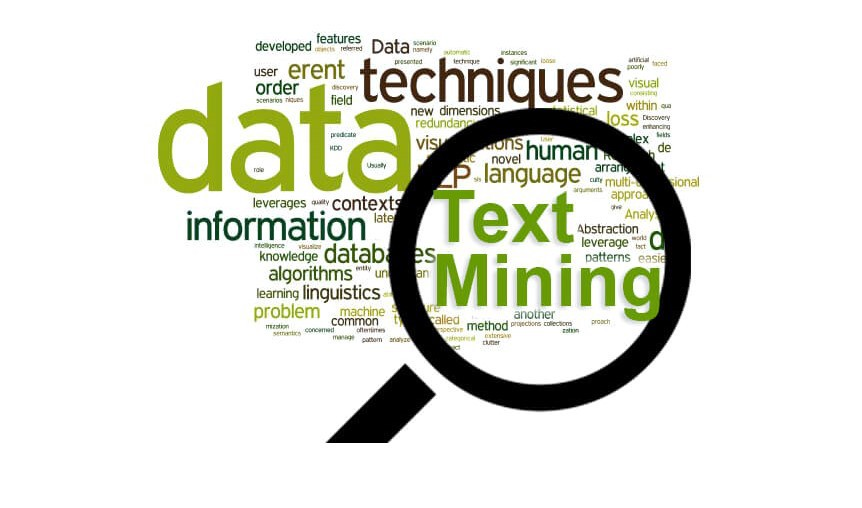
\includegraphics[width = 0.5 \textwidth]{fig31.jpg}}
\caption{Text mining.}
\label{fig31}
\end{figure}

Se estima que el 80\% de la información relevante para una empresa viene de algún tipo de datos no estructurados, los cuales están formados, en gran parte, por texto. Por ejemplo, podemos encontrar información relevante en e-mails, informes e, incluso, artículos en las redes sociales.



\subsection{Ventajas del Text Analytics}

\subsubsection{Estado real de la empresa}

En los textos redactados también entran los informes periódicos o los balances, por citar dos ejemplos. Repasando la información recopilada resulta más fácil descubrir el estado real de la empresa, por lo que es más sencillo adelantarse a posibles problemas y tomar decisiones acertadas \cite{Ormeno}.

\subsubsection{Opiniones en los clientes}

En el repaso de los textos también se incluyen las opiniones de los clientes, por lo que es posible determinar cuáles son los errores que se están cometiendo. Además, es posible personalizar la oferta comercial al entender mejor cuáles son sus necesidades o qué demanda exactamente.

\subsubsection{Creación de etiquetas}

Contribuye a la creación de etiquetas que clasifiquen los productos a la venta dependiendo de su material, fabricante o peculiaridades, entre otros factores.

\begin{figure}[htbp]
\centerline{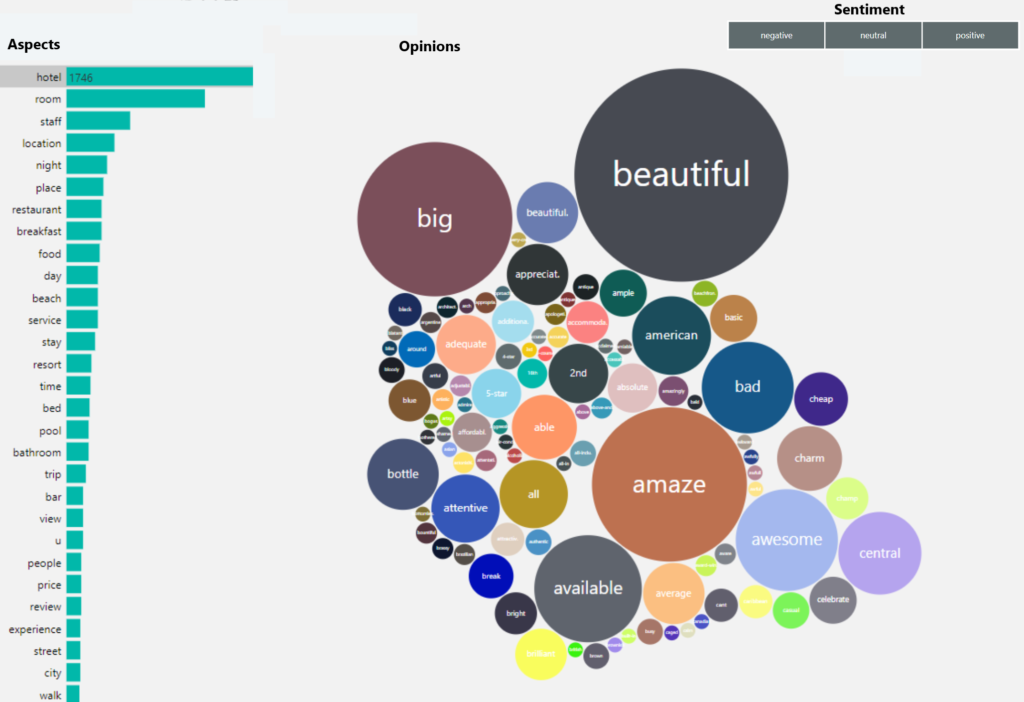
\includegraphics[width = 0.5 \textwidth]{fig44.png}}
\caption{Ejemplo de etiquetas.}
\label{fig44}
\end{figure}

Text Analytics (Text MIning), lo que parece ser una disciplina asociada a la Business Intelligence y al Big Data, es también una herramienta para predecir tendencias, conocer mejor a la clientela y, definitivamente, repasar la información pasada dándole su valor para convertirla en la más útil para el futuro.

\subsubsection{Speech Recognition}

El Reconocimiento Automático de Voz (RAH) o Reconocimiento Automático de Voz es un tema de inteligencia artificial, que tiene como objetivo realizar la comunicación de voz entre humanos y computadoras.

\begin{figure}[htbp]
\centerline{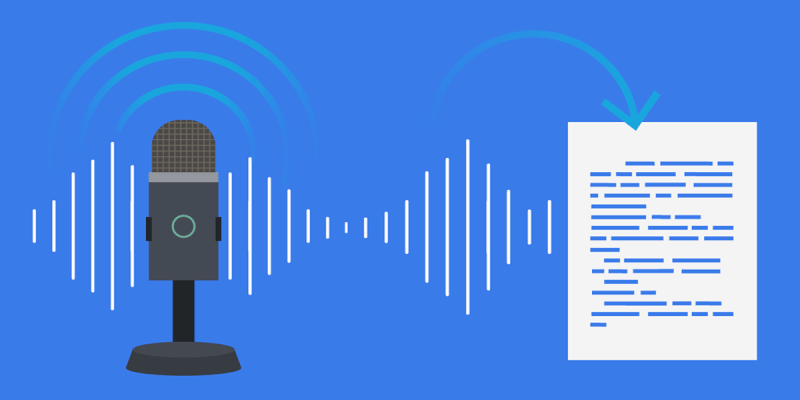
\includegraphics[width = 0.5 \textwidth]{fig43.png}}
\caption{Reconocimiento de voz.}
\label{fig43}
\end{figure}

\subsubsection{En salud}

Encontrar información rápidamente a partir de registros médicos.
Las enfermeras pueden solicitar información administrativa, como el número de pacientes en un piso y el número de unidades disponibles.
En casa, los padres pueden preguntar por los síntomas comunes de las enfermedades, cuándo deben ir al médico y cómo cuidar a un niño enfermo.

\begin{figure}[htbp]
\centerline{
\includegraphics[width = 0.5 \textwidth]{fig38.jpg}}
\caption{Servicios cognitivos en salud.}
\label{fig38}
\end{figure}

\subsubsection{En banca}

Solicite información sobre su saldo, transacciones y hábitos de gasto sin tener que abrir su teléfono celular.
Realizar pagos.
Reciba información sobre su historial de transacciones.

\begin{figure}[htbp]
\centerline{
\includegraphics[width = 0.5 \textwidth]{fig42.jpg}}
\caption{Servicios cognitivos en banca.}
\label{fig42}
\end{figure}

\subsubsection{Con Internet de las cosas}

Aplicación de asistentes digitales en coches: 
Escuche mensajes con manos libres.
Controla tu radio.
Ayudar con la guía y la navegación.
Responder a los comandos de voz.

\begin{figure}[htbp]
\centerline{
\includegraphics[width = 0.5 \textwidth]{fig33.jpg}}
\caption{Servicios cognitivos en IoT.}
\label{fig33}
\end{figure}

\subsubsection{Traducción}

La inteligencia artificial (IA) puede ayudar a simplificar la comunicación al traducir texto o habla entre idiomas, lo que ayuda a eliminar las barreras a la comunicación entre países y culturas.

\begin{figure}[htbp]
\centerline{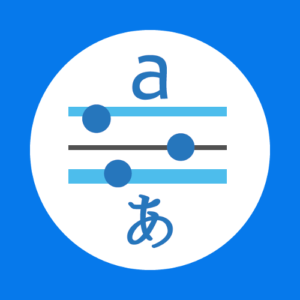
\includegraphics[width = 0.5 \textwidth]{fig37.png}}
\caption{Traductores y servicios cognitivos.}
\label{fig37}
\end{figure}

Traductor, parte de Servicios cognitivos Azure, es una nube basada en traducción automática servicio de apoyo a 90 idiomas y dialectos. Translator se puede utilizar para crear aplicaciones, sitios web, herramientas o cualquier solución que requiera soporte multilingüe.
¿Cómo funciona la traducción de voz?
Para traducir correctamente el discurso “fuente” de un idioma a otro idioma “target”, el sistema pasa por un proceso de cuatro pasos:

Reconocimiento de voz, convertir audio en texto.

TrueText: una tecnología de Microsoft que normaliza el texto para que sea más apropiado para la traducción.

Traducción a través del motor de traducción de texto descrito anteriormente, pero sobre modelos de traducción especialmente desarrollados para conversaciones habladas en la vida real.
Texto a voz, cuando sea necesario, para producir el audio traducido.

\begin{figure}[htbp]
\centerline{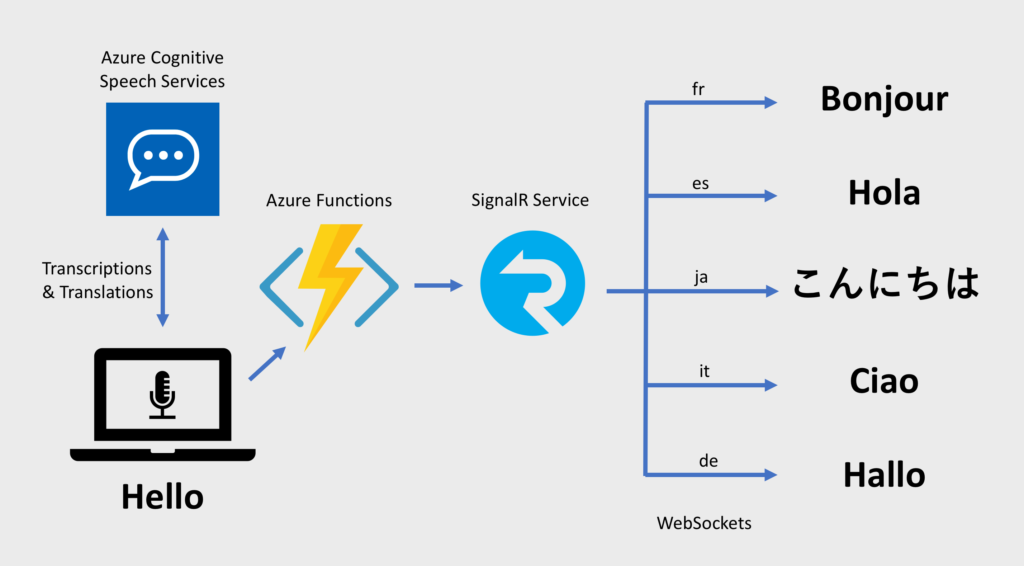
\includegraphics[width = 0.5 \textwidth]{fig32.png}}
\caption{Arquitectura de un traductor.}
\label{fig32}
\end{figure}

\subsubsection{Language Understanding (LUIS)}

Language Understanding Intelligent Service (LUIS, por sus siglas en inglés) utiliza el aprendizaje automático para permitir a los desarrolladores crear aplicaciones que puedan entender el lenguaje natural de los usuarios para extraer su significado y comprender lo que la persona quiere. En pocas palabras, tener la habilidad de entender de una manera clara la forma en que las personas se comunican en su cotidianidad.

\begin{figure}[htbp]
\centerline{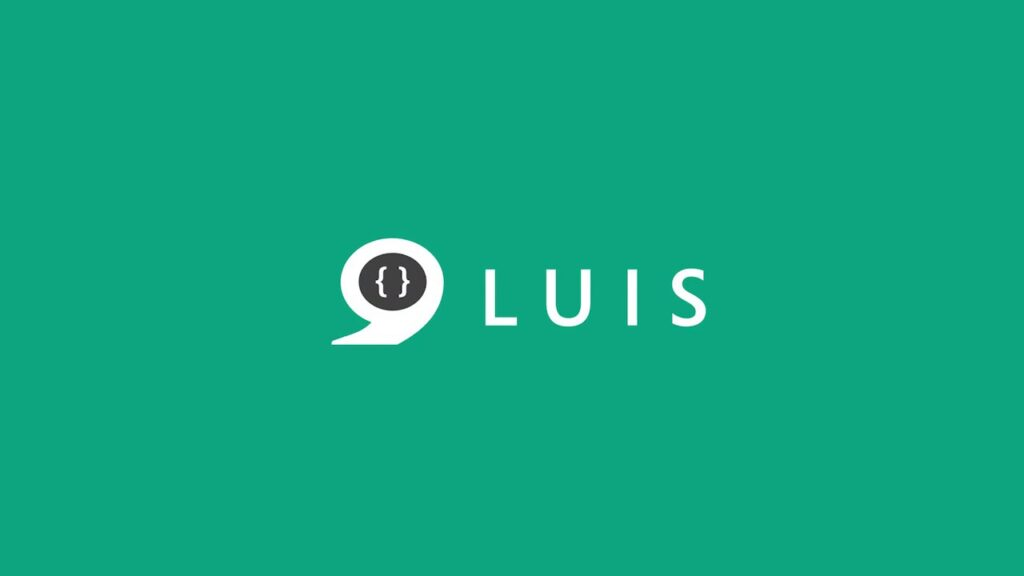
\includegraphics[width = 0.5 \textwidth]{fig39.jpg}}
\caption{LUIS}
\label{fig39}
\end{figure}

LUIS añade comprensión natural del lenguaje a tus aplicaciones. Está diseñado para identificar información valiosa en conversaciones, interpretar los objetivos del usuario e identificar información relevante en las oraciones para comunicarse en un lenguaje natural y de alta calidad.

LUIS está en constante aprendizaje. El aprendizaje de refuerzo se usa para mejorar continuamente la calidad de los modelos de procesamiento del lenguaje natural.

Una vez que el modelo comienza a procesar la entrada, la comprensión del idioma empieza su aprendizaje activo permitiendo así actualizar y mejorar constantemente el modelo.

Chatbot de información: Este Bot informacional puede responder preguntas definidas en un conjunto de conocimientos o preguntas frecuentes usando Azure Search.

Dispositivos de IoT: Se pueden crear interfaces de conversación con todos sus dispositivos accesibles en Internet.

\begin{figure}[htbp]
\centerline{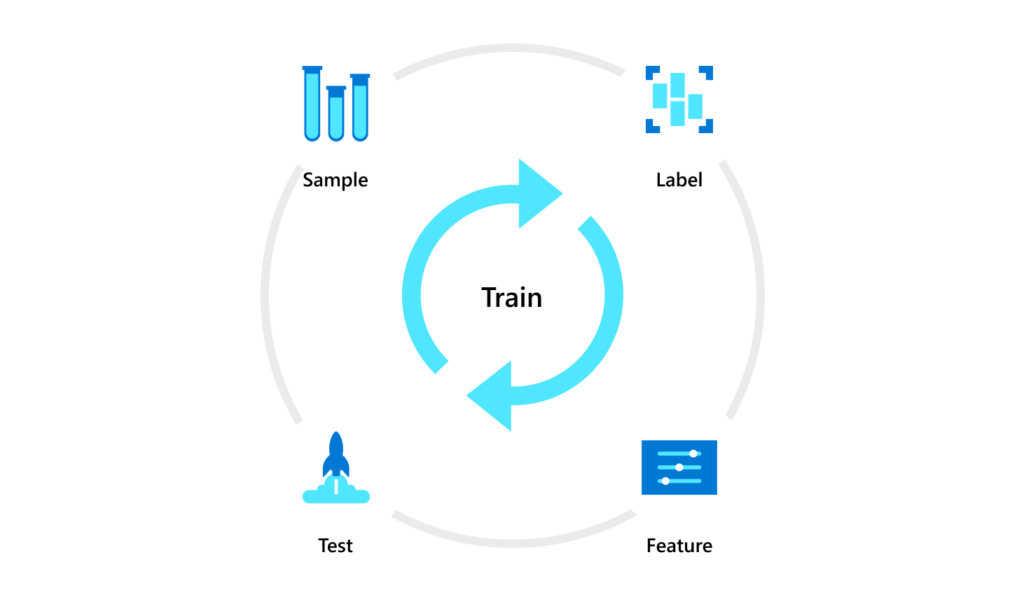
\includegraphics[width = 0.5 \textwidth]{fig40.png}}
\caption{Funcionamiento de LUIS}
\label{fig40}
\end{figure}

\subsubsection{Chatbot: ¿Qué es, para qué sirve y cómo funcionan?}

Hoy en día Internet está muy masificado, resulta difícil destacar entre tanta información. Las empresas buscan los canales digitales para llamar la atención y tener contacto con los usuarios. Los consumidores aceptan este hecho y prefieren tener el contacto con las empresas a través de mensajes.
Adiós a los medios digitales de antes, los medios tradicionales como los call center, por ejemplo, ya están obsoletos. La solución que se ha planteado para hacer feliz tanto a las empresas como a los consumidores son: los chatbots.

\begin{figure}[htbp]
\centerline{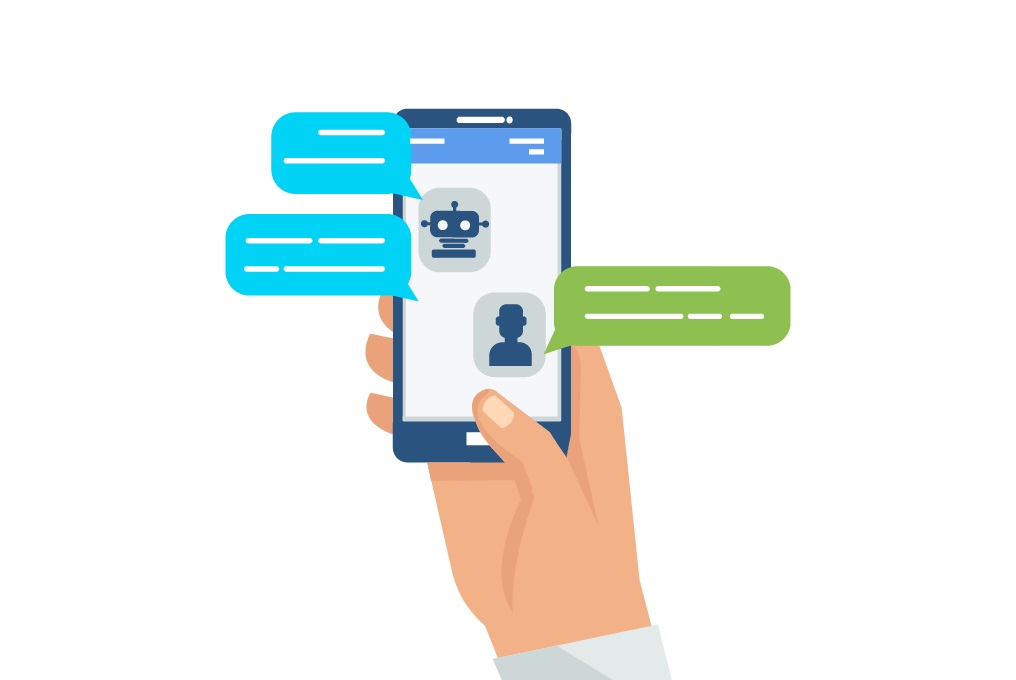
\includegraphics[width = 0.5 \textwidth]{fig41.jpg}}
\caption{Funcionamiento de un chatbot.}
\label{fig41}
\end{figure}

\subsubsection{¿Qué es un chatbot?}

De manera sencilla y comprensible podemos definir un chatbot como un asistente que se comunica con los usuarios a través de mensajes de texto. En muchas otras ocasiones, toma forma convirtiéndose en un compañero virtual que se integra en sitios web, aplicaciones, conversando y ayudando a los usuarios \cite{Peris}.

Se trata de una tecnología que permite al usuario mantener una conversación a través de un software que se integra en un determinado sistema de mensajería, como, por ejemplo: Facebook, Twitter, Telegram, Whatsapp, etc.
El sistema está programado para que interactúe con el cliente y le resuelva dudas, pero sin que haya una persona física contestando. Tienen la ventaja de que están disponibles siempre para resolver las dudas de los usuarios que quieran contactar contigo a cualquier hora del día.

Por lo tanto, estamos hablando de una herramienta que interactúa de manera automática con usuarios y potenciales clientes con el fin de guiarles hacia la acción deseada (conversión).

Los algoritmos desarrollados por la inteligencia artificial y de aprendizaje automático permiten que los chatbots sean capaces de aprender. Pueden llegar a intuir los hábitos y entender los gustos y preferencias de los usuarios.

Existen muchos tipos de chats en vivo, algunos de ellos ofrecen una experiencia tan auténtica, en la que es muy difícil determinar si el que contesta es un robot virtual o un ser humano.

\subsubsection{¿Por qué han aparecido los chatbots?}

Actualmente, estamos viviendo una transformación digital y un momento en el que los datos son un valor importante para las empresas. Es aquí donde entra el papel tan relevante de los chatbots, puesto que son softwares diseñados con el fin de poder conectar de manera personalizada con los usuarios, resolviendo sus dudas, aportando valor para ellos, pero disminuyendo enormemente el gasto que esta interacción supondría para la empresa si se realizara con representantes humanos. El resultado es un ahorro en tiempo y dinero para la empresa y una mayor comodidad y rapidez para el usuario.

\subsubsection{¿Cómo funcionan los chatbots?}

Para comprender el funcionamiento de un chatbot debemos primero entender qué es un bot. Un bot es un software de inteligencia artificial con la característica diferencial de ser capaz de realizar una serie de tareas por su cuenta, sin la ayuda del ser humano. 

El chatbot es un tipo de bot que interactúa con el usuario manteniendo conversaciones sencillas, pero que también puede convertirse en un sofisticado software a medida que procesan información, y aprender y evolucionar con el fin de ofrecer niveles de personalización cada vez más elevados. Siri y Cortana serían los ejemplos más conocidos de chatbot.

Los chatbots son utilizados por las empresas principalmente para llevar a cabo tareas y funciones de atención al cliente: realizar pedidos automáticos, comunicar incidencias técnicas, pedir información sobre un determinado producto o servicio, etc. Pero también tienen su uso en los procesos internos de la propia empresa, como pueden ser los pedidos de suministros internos, las programaciones en calendarios o facilitar el proceso de entrada de nuevos trabajadores.

La operatividad de los chatbots tiene lugar en las aplicaciones de mensajería, incorporando para ello un interfaz conversacional.
Vale la pena señalar que entender a los humanos no es fácil para una máquina. La forma sutil y matizada en la que nos comunicamos es una tarea muy compleja de recrear artificialmente, por lo que los chatbots utilizan varios principios del lenguaje natural:

\subsection{Procesamiento del Lenguaje Natural (PLN)}

El Procesamiento de Lenguaje Natural se utiliza para dividir la entrada del usuario en oraciones y palabras. También amplia el significado del texto a través de una serie de técnicas como, por ejemplo: Convirtiendo todo a minúsculas o corrigiendo errores ortográficos antes de determinar el significado de la palabra. En esta etapa, es donde también se consideran otros factores tales como las emociones del usuario.

\subsubsection{Comprensión del Lenguaje Natural (CLN)}

La comprensión del lenguaje natural ayuda al chatbot a entender lo que el usuario ha dicho, las herramientas que utiliza son tales como léxicos, sinónimos y temas. Estas herramientas son usadas en conjunto como algoritmos o reglas para construir el diálogo que le indicará al chatbot cómo debe responder de la mejor manera posible.

\subsubsection{Generación de Lenguaje Natural (GNL)}

Ofrecer una experiencia al cliente memorable, personalizada e ir más allá de brindar respuestas prefabricadas, requiere la generación de lenguaje natural. El chatbot puede consultar repositorios de datos y así, utilizar esa información para crear una respuesta.

La tecnología de IA Conversacional lleva el PLN y la CLN al siguiente nivel, permitiendo a las empresas puedan crear sistemas de diálogo avanzados.
Usan memorias y datos de preferencias personales y la propia comprensión contextual del chat para ofrecer una interfaz de lenguaje natural realista y atractiva.

\subsubsection{Ventajas de los chatbots}

Las principales ventajas del uso de chatbots por parte de las empresas son:

Permite ahorrar costes en formación y personal del departamento de atención al cliente.

Permite atender las principales dudas y gestiones de los usuarios de manera rápida.

Abre la posibilidad a escalar y a su vez ofrecer una atención personalizada, ya que se depende menos del esfuerzo humano, pero no es necesario usar modelos estandarizados para poder dar respuesta.

Un chatbot posibilita una interacción muy ágil con el cliente.

En ciertos casos, el chatbot puede llegar a proporcionar experiencias muy agradables y cómodas al usuario.

Otra ventaja es la rápida mejora de las posibilidades y el nivel de sofisticación de los softwares de inteligencia, llegando a simular con gran realismo conversaciones bastante complejas.

Se trata de una tecnología que está abriendo nuevas fuentes de ingresos y oportunidades de negocio. Por este motivo, desarrolladores de software, marcas y empresas se están volcando en ofrecer sus servicios a través de este canal.
A muchas personas les resulta más sencillo y cómodo hablar con un robot de voz que con la persona encargada de atenderle telefónicamente.
Tipos de chatbots que existen en el mercado
Actualmente, existen distintos tipos de chatbots que procesan la información y pueden dar respuesta a solicitudes de distinta índole. A continuación, explicamos los dos tipos principales de chatbots \cite{Escote}.

\subsubsection{Tipo 1 - Chatbots orientados a tareas (declarativos)}

Son programas que generan respuestas automatizadas a las consultas que los usuarios puedan realizar y lo hacen de manera conversacional. Es por ello que son más aplicables a los departamentos de soporte, atención al cliente y servicio, pues las interacciones con estos chatbots son específicas y estructuradas.

Los ejemplos más claros de chatbots declarativos serían aquellos que se emplean en preguntas comunes como precios de productos concretos u horarios comerciales. Sus capacidades son bastante básicas, pero son los chatbots más utilizados.

Tipo 2 - Chatbots basados en datos y predictivos (conversacionales)
Son herramientas capaces de personalizar su respuesta basándose en el perfil de cada usuario y su comportamiento anterior. Estos son conscientes del contexto y aprenden con cada nueva situación. Además, aprovechan su comprensión del lenguaje natural para ofrecer recomendaciones e incluso llegar a anticiparse a las necesidades del usuario.



¿Cómo crear un chatbot?
No es necesario ser un experto para crear un chatbot y hay muchas herramientas que permiten hacerlo. Crear uno es similar a desarrollar una aplicación móvil y se puede enfocar a usos empresariales o a consumidores.
Los chatbots se pueden crear e ir enfocados a ciertas herramientas. Por ejemplo, puedes crear un Chatbot para Whatsapp para mejorar el Customer Service de tu negocio.
Entre las distintas herramientas que existen en el mercado, con HubSpot puedes crear un Chatbot gratis para implementarlo en la web de tu empresa y enfocarlo como una parte más de tu estrategia de marketing.
El chatbot de Facebook
Aunque Twitter y otras plataformas, como Telegram, también han empezado a incorporar funciones de chatbots a sus servicios de mensajería, lo cierto es que de momento Facebook puede considerarse la empresa referente en el desarrollo de sistemas basados en chatbots.

Dado que la mayoría de las empresas no disponen de recursos propios para elaborar chatbots, Facebook les está suministrando herramientas de API (interfaz de programación de aplicaciones) para que puedan crear sus propios softwares de inteligencia artificial personalizados y adaptados a sus necesidades.

En Facebook, los chatbots se encuentran integrados dentro de su aplicación Messenger. Ello permite realizar acciones como encargar un ramo de flores o pedir que la CNN nos mande un resumen de las noticias que más nos interesan en función de nuestros gustos e inquietudes.
Se trata de una funcionalidad enfocada a empresas y marcas que el propio Mark Zuckerberg se encargó de promocionar en el último congreso de desarrolladores F8, afirmando que los usuarios podrán hablar con los chatbots igual que lo harían con sus amigos.  
Además de facilitar la atención al cliente y mejorar la experiencia del usuario, una ventaja adicional del chatbot de Facebook son las nuevas posibilidades publicitarias. La red social Facebook dará la opción a las empresas de enviar anuncios con mensajes patrocinados a aquellos usuarios que, previamente, hayan iniciado de manera voluntaria una conversación por chatbot con la marca.
Preguntas y Respuestas
¿Cuáles son los mejores chatbot?
Entre los mejores chatbots que se encuentran el mercado están:
Aivo
Zendesk
Botslover
Messenger People
Son plataformas que se pueden usar tanto en webs como en herramientas de mensajería, ofrecen herramientas de análisis y te permiten gestionar desde un solo espacio todos los canales que ofreces a tus usuarios.
¿Cuál es el mejor chatbot en español?
HubSpot actualmente se posiciona como la mejor herramienta para configurar un chatbot en español, pues permite mantener conversaciones a gran escala en el propio sitio web y automatizar los procesos. Así, tu equipo se focaliza en las conversaciones más importantes o delicadas. Es perfecto para empezar, pues no requiere ningún conocimiento técnico y dispone de plantillas con la opción de personalizarlas para alinearlo con la voz de tu marca. Asimismo, ayuda a calificar los leads y ofrecerles respuestas rápidas y adecuadas a las preguntas técnicas frecuentes y a hacer un seguimiento de las conversaciones.
¿Cuál es el mejor chatbot gratis para WhatsApp?
Zendesk es una aplicación chatbot gratuita y muy buena para usar en WhatsApp, pues te permite personalizar los mensajes, hacer seguimiento de las conversiones y permite tener un registro de toda la información que se recoge con el chatbot.
¿Dónde se utilizan los chatbots?
Los chatbots se pueden usar en 2 tipos de enfoque: a nivel interno o para interactuar con los consumidores.
En el ámbito del servicio al consumidor, podemos emplear los chatbots en la propia página web para dar respuesta a las dudas que tenga el usuario, y en las aplicaciones de mensajería o redes sociales para automatizar las conversaciones y agilizar procesos.
A nivel interno lo podemos usar para automatizar pedidos de suministros y otras tareas comunes como actualización de contraseñas, alertas en las oficinas o incorporación de nuevos trabajadores.
¿Qué son los chatbots en un móvil Android?
Un chatbot en Android es un software encargado de dar respuesta a las consultas que los usuarios de una App puedan tener. En la misma aplicación se despliega un chat donde el usuario puede lanzar consultas y hablar directamente con la empresa de la aplicación. Es una manera de ofrecer el servicio dentro de la propia aplicación, sin tener que sacar al usuario fuera de ésta.
¿Puede un chatbot funcionar sin IA?
Existen chatbots sin IA que se crean desde cero y permiten realizar tareas muy parecidas a los chatbots con inteligencia artificial. Estos son efectivos a la hora de mejorar el servicio al cliente, pero no captan todas las necesidades del cliente, ya que solo resuelven las dudas en las que ha habido una previa configuración.
¿Existen chatbots gratuitos?
Existen chatbots gratuitos que pueden ser muy útiles para un negocio que está empezando; entre ellos podemos encontrar:
Plataforma Centribal, que en su versión gratuita permite crear, gestionar y entrenar un chatbot.
Live Chat, que permite centralizar todas las conversaciones de la web en un solo sitio.
Zendesk, que es muy sencilla de instalar y permite integrar todo tipo de soportes, desde chat hasta redes sociales.

La Influencia de los sistemas cognitivos en la empresa
Desde un punto de vista conceptual genérico, hay dos grandes beneficios asociados a la utilización de sistemas cognitivos en las empresas: 
1) la racionalización y automatización de procesos.
2) el enriquecimiento de procesos, productos y servicios.
Desde el punto de vista de los casos de uso, los sistemas cognitivos tienen aplicación en cualquier industria y área funcional. Efectivamente, se basan en el reconocimiento de patrones a partir del procesamiento de un gran conjunto de datos a una escala que está más allá de la capacidad humana, con lo que se pueden aplicar en muchos dominios – como, por ejemplo, análisis e investigación de fraudes, recomendación y automatización de procesos de venta, sistemas de investigación y recomendación de gestión de calidad, agentes de servicio automatizados, sistemas automatizados de inteligencia y prevención de amenazas, sistemas de búsqueda y acceso a contenidos, etc \cite{Malhado}.
Tomemos como ejemplo detallado el sourcing y procurement; en particular, el proceso de source to settle. Típicamente, el 20\% de la inversión se concentra en el 80\% de los proveedores. Hay muchas transacciones, pero el valor monetario total de cada uno es bajo en comparación con el total y hay muchos proveedores potenciales para los bienes, por lo que el riesgo de oferta es también bajo. La automatización del proceso final (desde el aprovisionamiento hasta la contratación) para estas transacciones rutinarias de bajo riesgo (a través de la aplicación del aprendizaje automático y el procesamiento del lenguaje natural) libera personal cualificado para concentrarse en la inversión y proveedores con mayor riesgo de suministro y coste financiero, así como en la gestión de las relaciones con los proveedores más críticos. Y para estos procesos menos rutinarios, el aprendizaje automático aumenta el proceso de sourcing mediante el monitoreo de señales que podrían conducir a una interrupción del suministro, asesorando al personal sobre las acciones correctivas disponibles y alternativas. Todo el proceso (tanto rutinario como no rutinario) se implementa a través de una combinación de automatización y enriquecimiento. Todo esto significa otra cosa: que uno de los grandes impactos de los sistemas cognitivos está en la fuerza de trabajo. Ellos van a cambiar la fuerza de trabajo de las empresas. Ya no sorprende a nadie la predicción de que la fuerza de trabajo del futuro será compuesta no solo por humanos, sino también por agentes virtuales.

¿Qué deberían estar haciendo las empresas en torno al tema Sistemas Cognitivos / IA?
Existen varios modelos de utilización de capacidades cognitivas en las empresas:
Agentes cognitivos dedicados que pueden ser involucrados en varios procesos de la empresa.
Funcionalidades embebidas en el software empresarial.
Plataformas de servicios (típicamente consumidos a través de la nube).
Queda claro que cualquiera que sea la combinación o arquitectura seleccionada por cada empresa, esta implicará una revisión de sus procesos. El TI y el negocio tendrán que trabajar conjuntamente para evaluar el valor de la nueva inteligencia proporcionada por el software e identificar los casos de implementación prioritaria. Además, las empresas deberían estar buscando a sus proveedores de tecnología para ver cómo las capacidades cognitivas / IA están siendo incluidas en los roadmaps de productos y cómo podrán hacer uso de dichas capacidades. Y los departamentos de TI deberán estar aprendiendo sobre las diversas plataformas de software cognitivo / AI disponibles y comenzar a probar algunas nuevas aplicaciones en ellos. Algunas de estas plataformas son gratuitas para uso en desarrollo. Las organizaciones de TI necesitan crear experiencia interna en estas áreas junto con la ciencia de datos y Big Data.

Servicios cognitivos y su impacto en la empresa Microsoft
Los servicios cognitivos de Microsoft son API basadas en la nube que puede usar en aplicaciones de inteligencia artificial (AI) y flujos de datos. Proporcionan modelos previamente entrenados que están listos para usarlos en cualquier aplicación, no requieren datos ni entrenamiento del modelo por su parte. Los servicios cognitivos los desarrolla el equipo de inteligencia artificial e investigación de Microsoft y aprovechan los algoritmos de aprendizaje profundo más recientes. Se consumen a través de las interfaces de REST de HTTP. Además, hay disponibles SDK para muchos marcos de desarrollo de aplicaciones comunes \cite{Microsoft2022}.
Los servicios cognitivos incluyen:
Análisis de texto
Visión del equipo
Análisis de vídeo
Reconocimiento y generación de voz
Comprensión del lenguaje natural
Búsqueda inteligente
Ventajas principales:
Con un esfuerzo mínimo de desarrollo se logran servicios de AI de última generación.
Fácil integración en aplicaciones a través de interfaces de REST de HTTP.
Compatibilidad integrada para consumir servicios cognitivos en Azure Data Lake Analytics.
Consideraciones:

Solo está disponible a través de Internet. Por lo general se requiere conectividad a Internet. Una excepción es Custom Vision Service, cuyo modelo entrenado se puede exportar para la predicción en dispositivos y en el borde de IoT.

Aunque se admite una personalización considerable, es posible que los servicios disponibles no se ajusten a todos los requisitos de análisis predictivo.

¿Qué opciones tiene al elegir entre los servicios cognitivos?
En Azure, existen docenas de servicios cognitivos disponibles. La lista actual de ellos está disponible en un directorio y están clasificados por el área funcional que admiten:
Visión
Identifique y analice el contenido de imágenes y vídeos
API de reconocimiento facial: Detecte e identifique a personas y emoticonos en las imágenes.

Computer Vision: Analice el contenido de imágenes y vídeos.

Custom Vision: Personalice el reconocimiento de imágenes para adaptarlo a sus necesidades empresariales.
Voz 
Mejore las experiencias de los clientes con Cognitive Service para voz:
Speech to Text: Transcriba la vox en texto legible en el que se puedan realizar búsquedas.

Text to Speech: Convierta el texto en un lenguaje más real para obtener interfaces más naturales.

Speech Translation: Integre fácilmente traducción de voz en tiempo real en sus aplicaciones.

Speaker Recognition: Identifique a las personas que hablan y compruébelo basándose en audio.
Decisión
Tome decisiones más inteligentes en menos tiempo
Anomaly Detector: Realice una identificación temprana de los posibles problemas.

Content Moderator: Detecte contenido potencialmente ofensivo o no deseado.

Personalizer: Cree experiencias personalizadas muy completas para cada usuario.
Lenguaje
Entienda las conversaciones y el texto no estructurado con Cognitive Service para lenguaje:
Reconocimiento de entidades: Identifique los términos de uso común y específicos del dominio \cite{Molnar2019}.

Análisis de opiniones: Detecte automáticamente sentimientos y opiniones a partir de texto.

Respuesta a preguntas: Cree una capa conversacional de preguntas y respuestas sobre los datos.

Language Understanding: Incorpore reconocimiento del lenguaje natural a sus aplicaciones, bots y dispositivos IoT.

Translator Text: Detecte y traduzca más de 100 idiomas y dialectos.
OpenAI
Modelos de lenguaje dinámicos para mejorar las aplicaciones
OpenAI Service: Aplique modelos de lenguaje avanzados a una gran variedad de casos de uso.

Principales criterios de selección
Para restringir las opciones, empiece por responder a estas preguntas:

¿Con qué tipo de datos trata? Puede limitar las opciones en función del tipo de datos de entrada con el que trabaje. Por ejemplo, si la entrada es texto, seleccione uno de los servicios que tenga un tipo de entrada de texto.

¿Tiene los datos necesarios para entrenar un modelo? En caso afirmativo, considere los servicios personalizados que le permiten entrenar sus modelos subyacentes con los datos que proporcione, con el fin de mejorar la precisión y el rendimiento \cite{Blanco}.

Matriz de funcionalidades
En las tablas siguientes se resumen las diferencias clave en cuanto a funcionalidades.

Usa modelos creados previamente
\begin{table}[]
\begin{tabular}{| p{0.15\linewidth} | p{0.15\linewidth} | p{0.5\linewidth} |}
\hline
\textbf{Capacidad} &
  \textbf{Tipo de entrada} &
  \textbf{Principal ventaja} \\ \hline
Text Analytics API &
  Texto &
  Evalúe las opiniones y temas para comprender lo que los usuarios quieren. \\ \hline
Entity Linking API &
  Texto &
  Alimente los vínculos de datos de su aplicación con el reconocimiento y la anulación de ambigüedades de las entidades con nombre. \\ \hline
Language Understanding Intelligent Service (LUIS) &
  Texto &
  Enseñe a las aplicaciones a entender los comandos de los usuarios. \\ \hline
Servicio QnA Maker &
  Texto &
  Convierta la información con formato de preguntas frecuentes en respuestas conversacionales por las que sea fácil navegar. \\ \hline
Linguistic Analysis API &
  Texto &
  Simplifique conceptos complejos del lenguaje y analice el texto. \\ \hline
Servicio Knowledge Exploration &
  Texto &
  Permita experiencias de búsqueda interactiva a través de datos estructurados mediante entradas en lenguaje natural. \\ \hline
Web Language Model API &
  Texto &
  Use modelos de lenguaje predictivos entrenados con datos de escala web. \\ \hline
Academic Knowledge API &
  Texto &
  Descubra la riqueza del contenido académico de Microsoft Academic Graph rellenado por Bing. \\ \hline
Bing Autosuggest API &
  Texto &
  Proporcione a su aplicación opciones de sugerencias automáticas inteligentes para las búsquedas. \\ \hline
Bing Spell Check API &
  Texto &
  Detecte y corrija errores ortográficos en las aplicaciones. \\ \hline
Translator Text API &
  Texto &
  Servicio de traducción automática. \\ \hline
Recommendations API &
  Texto &
  Prediga y recomiende los artículos que sus clientes quieren. \\ \hline
Bing Entity Search API &
  Texto (consulta de búsqueda web) &
  Identifique y amplíe la información de las entidades desde la web. \\ \hline
Bing Image Search API &
  Texto (consulta de búsqueda web) &
  Busque imágenes. \\ \hline
Bing News Search API &
  Texto (consulta de búsqueda web) &
  Busque noticias. \\ \hline
Bing Video Search API &
  Texto (consulta de búsqueda web) &
  Busque vídeos. \\ \hline
Bing Web Search API &
  Texto (consulta de búsqueda web) &
  Obtenga detalles mejorados de la búsqueda de miles de millones de documentos web. \\ \hline
Bing Speech API &
  Texto o voz &
  Convierta voz en texto, y viceversa. \\ \hline
Speaker Recognition API &
  Voz &
  Use la voz para identificar y autenticar a hablantes individuales. \\ \hline
Translator Speech API &
  Voz &
  Realice traducciones de voz en tiempo real. \\ \hline
\end{tabular}
\end{table}

\begin{table}[]
\begin{tabular}{| p{0.15\linewidth} | p{0.15\linewidth} | p{0.55\linewidth} |}
\hline
\textbf{Capacidad} &
  \textbf{Tipo de entrada} &
  \textbf{Principal ventaja} \\ \hline
Computer Vision API &
  Imágenes (o fotogramas de vídeo) &
  Convierta la información accionable de las imágenes, cree automáticamente la descripción de las fotos, derive etiquetas, reconozca a celebridades, extraiga texto y cree miniaturas precisas. \\ \hline
Content Moderator &
  Texto, imágenes o vídeo &
  Moderación automatizada de imágenes, texto y vídeo. \\ \hline
Emotion API &
  Imágenes (fotos con seres humanos) &
  Identifique la gama de emociones de los seres humanos. \\ \hline
Face API &
  Imágenes (fotos con seres humanos) &
  Detecte, identifique, analice, organice y etiquete las caras en las fotos. \\ \hline
Video Indexer &
  Vídeo &
  Información acerca del vídeo, como la opinión, transcriba la voz, traduzca la voz, reconozca caras y emociones, y extraiga las palabras clave. \\ \hline
\end{tabular}
\end{table}